\documentclass[11pt,a4paper]{article}

\usepackage[margin=2.2cm]{geometry}
\usepackage{booktabs}
\usepackage{graphicx}
\usepackage{amsmath}
\usepackage{amssymb}
\usepackage{xcolor}
\usepackage[labelfont=bf,font=small]{caption}
\usepackage[hidelinks]{hyperref}
\usepackage{enumitem}

\definecolor{accent}{HTML}{2a78d6}
\definecolor{good}{HTML}{1f8a54}
\definecolor{bad}{HTML}{cf3a4e}
\definecolor{ink}{HTML}{0b0b0b}
\setlist[itemize]{leftmargin=1.4em,itemsep=2pt,topsep=3pt}
\setlist[enumerate]{leftmargin=1.6em,itemsep=4pt,topsep=3pt}
\newcommand{\num}[1]{\texttt{#1}}

\title{\vspace{-1.6cm}\textbf{Feature Regularisation of a Tree Encoding\\
under a Logistic-Regression Head}}
\author{TKCE project \\ \small Experiment report}
\date{\small 26 September 2026}

\begin{document}
\maketitle
\vspace{-0.7cm}

\begin{center}
\fbox{\begin{minipage}{0.95\textwidth}
\small\textbf{Summary.} With the classifier fixed to a scikit-learn logistic
regression, twenty-one runs covering eighteen distinct feature-regularisation
configurations were carried out on the \emph{credit} dataset. \textbf{Test AUC is essentially invariant across all of
them} (range \num{0.8424}--\num{0.8464} against a baseline of \num{0.8457}),
while the \textbf{train-minus-validation gap falls by a factor of more than ten}
(\num{0.0972} down to \num{0.0092}). The most efficient configuration keeps only
the three shallowest tree layers: \textbf{700 of 5{,}401 bits}, test AUC
\num{0.8460}, overfitting gap \num{0.0240}, and a fit that is roughly fifteen
times faster. \textbf{Depth-targeted noise gave no advantage over uniform noise
of the same budget.}
\end{minipage}}
\end{center}

\section{Goal of the experiment}

A previous experiment established that a plain logistic regression on the
out-of-bag-honest tree encoding reaches test AUC \num{0.8467} on \emph{credit},
against a LightGBM ceiling of \num{0.8453} and \num{0.8475} for a
2.44-million-parameter TabResNet. The neural network therefore contributed
nothing measurable, and the result lives entirely in the features.

The classifier was consequently fixed to a logistic regression, which is the
case of interest: overfitting is far milder than in the network, and the
tree-encoding features already perform on par with the gradient-boosted
baselines. All remaining experimentation moves to the \emph{features}. This
report asks four questions, following the directions set for this round:

\begin{enumerate}
  \item Does adding noise to the encoding, at various levels, reduce
        overfitting, and at what cost in accuracy?
  \item Does noise that \emph{increases with the depth} of the split outperform
        uniform noise of the same total budget? Deeper splits are fitted on
        fewer training rows and should be the least trustworthy.
  \item What happens when the deepest layers are deleted outright, and then the
        remaining layers are perturbed with a depth-increasing rate?
  \item How much of the encoding is actually needed, tested by keeping only the
        first three layers (depths 0, 1 and 2)?
\end{enumerate}

\section{Dataset}

\begin{table}[h]\centering\small
\begin{tabular}{ll}
\toprule
\textbf{Property} & \textbf{Value}\\
\midrule
Dataset & \emph{credit}, OpenML task \num{361055} (Grinsztajn tabular benchmark)\\
Task & binary classification: serious payment delinquency within two years\\
Rows used & \num{16000}, split \num{11200} train / \num{2400} validation / \num{2400} test\\
Split & stratified random, fixed seed \num{0}\\
Features & 10 numerical (age, income, debt ratio, credit-line and late-payment counts, \dots)\\
Target balance & approximately 50/50 by the benchmark's preprocessing\\
Preprocessing & features standardised using training-split statistics only\\
Known leakage & none; this dataset is not on the leaky-dataset list\\
\bottomrule
\end{tabular}
\end{table}

\noindent\textbf{Reference baselines} fitted on the raw features of the same
split:

\begin{table}[h]\centering\small
\begin{tabular}{lcc}
\toprule
\textbf{Model} & \textbf{Test AUC} & \\
\midrule
LightGBM & \textbf{\num{0.8453}} & $\leftarrow$ the ceiling used throughout\\
XGBoost & \num{0.8375} & \\
Random Forest & \num{0.8370} & \\
\bottomrule
\end{tabular}
\end{table}

\section{Architecture}

The model has two stages. The first is fixed and fitted once; the second is the
only thing that learns.

\paragraph{Stage 1: the tree encoding (fixed).}
A random forest of \num{100} trees with \num{max\_depth = 6} and
\num{min\_samples\_leaf = 5} is fitted on the training split. Every
\emph{internal} node of every tree contributes one binary feature, called a
\emph{bit}: it is $1$ if the row satisfies that node's test $x_f \le t$ and $0$
otherwise. Concatenating over all nodes of all trees gives \textbf{5{,}401
bits}. The forest is never updated afterwards; it is a feature map, not a
predictor.

\begin{table}[h]\centering\small
\begin{tabular}{lrrrrrrr}
\toprule
\textbf{Depth of split} & 0 & 1 & 2 & 3 & 4 & 5 & \textbf{total}\\
\midrule
Bits & 100 & 200 & 400 & 780 & 1{,}455 & 2{,}466 & \textbf{5{,}401}\\
Share of encoding & 1.9\% & 3.7\% & 7.4\% & 14.4\% & 26.9\% & 45.7\% & 100\%\\
Median training rows per split & \multicolumn{3}{c}{$\approx 2{,}355$ for depths 0--2}
  & \multicolumn{3}{c}{$\approx 133$--$208$ for depths 3--5} & \\
\bottomrule
\end{tabular}
\caption{Almost half the encoding sits in the single deepest layer, and those
splits are fitted on an order of magnitude fewer rows than the shallow ones.
This distribution is why deletion is specified by \emph{layer} rather than by a
percentage.}
\end{table}

\paragraph{Out-of-bag honesty.}
The forest was fitted using the training labels, so a training row's bits from
trees whose bootstrap sample \emph{contained} that row are contaminated: those
splits were partly carved to classify that very row. Test rows have no such
trees. To remove this asymmetry, each training row keeps only the bits of trees
for which it was out-of-bag (on average \textbf{36.8 of 100} trees), the rest
are zeroed, and the survivors are rescaled by $T/|\mathrm{OOB}|$ so expected
magnitudes match. Validation and test rows use all \num{100} trees. This
protocol is held fixed in every arm of this report.

\paragraph{Stage 2: the head (the only trained component).}
\[
\Pr(y=1 \mid b) \;=\; \sigma\!\left(w^{\!\top} b + c\right),
\qquad \sigma(z) = \frac{1}{1+e^{-z}},
\]
a scikit-learn \texttt{LogisticRegression}: one weight per bit, \emph{no hidden
layer and no nonlinearity}. There is nothing between the encoding and the
decision.

\section{Training strategy}

\paragraph{A convex fit, so no result can be blamed on the optimiser.}
The objective
\[
\min_{w,c}\;\; \tfrac{1}{2}\lVert w \rVert_2^2
\;+\; C \sum_{i=1}^{n} \log\!\left(1 + \exp\!\left(-y_i (w^{\!\top} b_i + c)\right)\right)
\]
is convex, and the solver (L-BFGS, \num{max\_iter = 2000}) returns the global
optimum. There is no learning rate, no epoch count, no batch size and no
initialisation anywhere in this experiment.

\paragraph{The penalty is held constant at $C = 0.01$.}
$C$ multiplies only the data-fitting term, so a \emph{small} $C$ means
\emph{strong} regularisation; in the textbook form $\sum \text{loss} + \lambda
\lVert w\rVert^2$ this is $\lambda = 1/(2C)$. It is deliberately \textbf{not}
re-tuned per arm: doing so would leave any score change attributable either to
the features or to a differently tuned penalty. Holding it fixed makes every
difference in the tables attributable to the features alone. For reference, an
earlier sweep found $C = 0.001$ better by \num{0.0008} on validation, which is
far inside the measurement noise.

\paragraph{How noise is applied to a convex solver.}
A mini-batch trainer can draw fresh flips at every batch, which is what makes
noise a \emph{regulariser} rather than one corrupted dataset. A convex solver
sees a single fixed matrix, so the equivalent used here is to stack
\textbf{three independently flipped copies} of the training rows and fit on all
of them together (\num{33600} rows), which approximates minimising the loss
\emph{averaged over the noise distribution}:
\[
\min_{w,c}\;\; \mathbb{E}_{\text{flips}}\big[\,\mathcal{L}(w,c;\tilde b)\,\big]
\;\;\approx\;\;
\frac{1}{K}\sum_{k=1}^{K} \mathcal{L}\big(w,c;\tilde b^{(k)}\big), \qquad K = 3 .
\]

\paragraph{Order of operations, and what evaluation sees.}
Flips are applied to the \emph{hard} $0/1$ bits and the out-of-bag mask is
applied afterwards, matching the earlier mini-batch implementation exactly.
\textbf{Validation and test always use clean, unflipped, all-trees bits.} A
deleted bit is removed as a column and its flip probability is forced to zero,
so a flip can never resurrect a feature that was deleted on purpose.

\paragraph{How overfitting is measured.}
The reported gap is
\[
\text{gap} \;=\; \mathrm{AUC}_{\text{train}}^{\text{clean}} - \mathrm{AUC}_{\text{validation}} ,
\]
where the training term is evaluated on \emph{clean} training bits, not on the
flipped matrix the model was fitted to. Scoring a noisy arm against its own
corrupted inputs makes the gap incomparable between arms and wrongly suggests
that noise increases overfitting; this correction was made before the runs
reported here.

\section{Experimental setup}

Four kinds of intervention, which compose. In all of them $d$ denotes the depth
of a split and $d_{\max} = 5$ is the deepest internal layer.

\begin{table}[h]\centering\small
\begin{tabular}{lll}
\toprule
\textbf{Intervention} & \textbf{Definition} & \textbf{Question}\\
\midrule
Uniform noise & $p(d) = p$ for every bit & noise at various levels\\
Depth ramp & $p(d) = P \cdot d / d_{\max}$; roots never flip & does more noise deeper help?\\
Deletion & drop all bits at the named depths & are the deep layers needed?\\
Combined & delete the deepest layers, then ramp the rest & the combined design\\
\bottomrule
\end{tabular}
\end{table}

\noindent\textbf{Matched budgets.} For a ramp with parameter $P$, the average
flip rate over all \num{5401} bits works out to
$\bar p = \sum_d n_d\,p(d) / N = 0.796\,P$ under this bit distribution. Every
ramp is therefore paired with a \emph{uniform} arm carrying the same average
rate, so the \emph{shape} of the noise can be separated from its \emph{amount}.
Without that pairing a ramp result cannot be interpreted.

\noindent\textbf{Bits only.} Every arm uses the tree bits alone, with no raw
features. Including the ten raw columns would give the model an unperturbed
shortcut (they reach \num{0.7785} by themselves under the same head), which
would mask the effect of the noise. One \texttt{x+tree} control is reported for
continuity.

\noindent\textbf{Scope.} Twenty-one runs were executed, covering eighteen
distinct feature configurations; two configurations appear once but serve as both
a noise level and a matched control, and three were refitted for stability.

\noindent\textbf{Stability.} Because the flips are random, three arms were
refitted three times with fresh noise. The spread of test AUC was
\num{0.0001}--\num{0.0002}, so single runs are reliable with respect to the
noise draw.

\section{Results}

\begin{table}[h]\centering\footnotesize
\begin{tabular}{llrrrrrr}
\toprule
\textbf{Arm} & \textbf{Depths kept} & \textbf{Bits} & $\bar p$ &
\textbf{Train} & \textbf{Val} & \textbf{Test} & \textbf{Gap}\\
\midrule
\multicolumn{8}{l}{\textit{Baseline}}\\
all bits, no perturbation & 0--5 & 5{,}401 & 0.0000 & 0.9465 & 0.8492 & 0.8457 & 0.0972\\
\midrule
\multicolumn{8}{l}{\textit{Uniform noise at various levels}}\\
uniform $p=0.05$ & 0--5 & 5{,}401 & 0.0500 & 0.9212 & 0.8490 & 0.8455 & 0.0722\\
uniform $p=0.08$ & 0--5 & 5{,}401 & 0.0800 & 0.9100 & 0.8490 & 0.8456 & 0.0611\\
uniform $p=0.10$ & 0--5 & 5{,}401 & 0.1000 & 0.9038 & 0.8487 & 0.8457 & 0.0551\\
uniform $p=0.16$ & 0--5 & 5{,}401 & 0.1600 & 0.8908 & 0.8488 & \textbf{0.8460} & 0.0420\\
uniform $p=0.20$ & 0--5 & 5{,}401 & 0.2000 & 0.8845 & 0.8487 & 0.8459 & 0.0359\\
uniform $p=0.40$ & 0--5 & 5{,}401 & 0.4000 & 0.8587 & 0.8457 & \textcolor{bad}{0.8433} & 0.0130\\
\midrule
\multicolumn{8}{l}{\textit{Depth-increasing noise}}\\
ramp $P=0.1$ & 0--5 & 5{,}401 & 0.0796 & 0.9109 & 0.8487 & 0.8457 & 0.0622\\
ramp $P=0.2$ & 0--5 & 5{,}401 & 0.1592 & 0.8921 & 0.8479 & \textcolor{bad}{0.8442} & 0.0442\\
ramp $P=0.5$ & 0--5 & 5{,}401 & 0.3979 & 0.8548 & 0.8456 & \textcolor{bad}{0.8424} & \textbf{0.0092}\\
\midrule
\multicolumn{8}{l}{\textit{Deleting the deepest layers}}\\
drop depth 5 & 0--4 & 2{,}935 & 0.0000 & 0.9162 & 0.8497 & \textbf{0.8464} & 0.0665\\
drop depths 4,5 & 0--3 & 1{,}480 & 0.0000 & 0.8898 & 0.8497 & 0.8460 & 0.0401\\
\textbf{keep depths 0--2 only} & 0--2 & \textbf{700} & 0.0000 & 0.8737 & 0.8497 & \textbf{0.8460} & \textbf{0.0240}\\
\midrule
\multicolumn{8}{l}{\textit{Deletion combined with a depth ramp}}\\
drop 5 + ramp $0.2$ & 0--4 & 2{,}935 & 0.0678 & 0.8854 & 0.8490 & 0.8458 & 0.0364\\
drop 4,5 + ramp $0.2$ & 0--3 & 1{,}480 & 0.0247 & 0.8771 & 0.8491 & 0.8459 & 0.0280\\
drop 4,5 + ramp $0.2$ rescaled & 0--3 & 1{,}480 & 0.0412 & 0.8718 & 0.8482 & \textcolor{bad}{0.8451} & 0.0236\\
keep 0--2 + ramp $0.2$ & 0--2 & 700 & 0.0185 & 0.8635 & 0.8473 & \textcolor{bad}{0.8437} & 0.0162\\
\midrule
\multicolumn{8}{l}{\textit{Controls}}\\
\texttt{x+tree} (bits $+$ 10 raw features) & 0--5 & 5{,}411 & 0.0000 & 0.9469 & 0.8494 & 0.8454 & 0.0975\\
LightGBM on raw features & --- & --- & --- & --- & --- & \num{0.8453} & ---\\
\bottomrule
\end{tabular}
\caption{All eighteen distinct configurations (\num{21} runs in total; three
arms were refitted for stability, and two configurations served double duty as
matched controls). $\bar p$ is the average flip probability over all
\num{5401} bits. Gap is train AUC minus validation AUC with the training term
measured on clean bits. Red marks the five arms that fall below the LightGBM
ceiling; four of the five involve a depth ramp.}
\end{table}

\begin{figure}[h]\centering
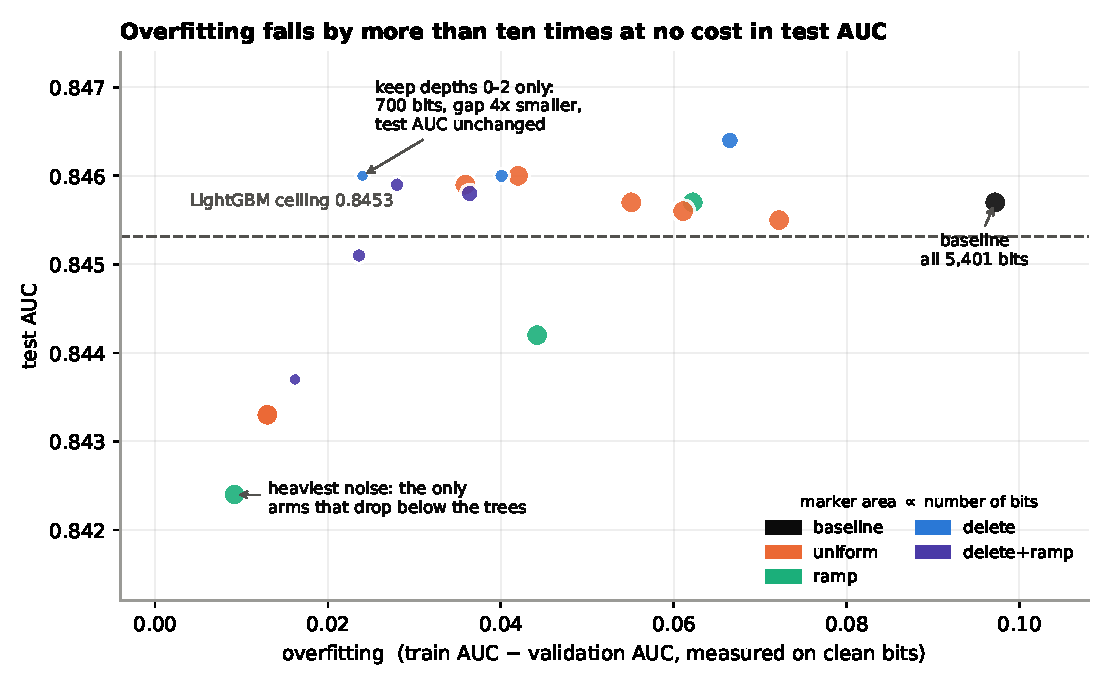
\includegraphics[width=0.93\textwidth]{fig1_tradeoff.pdf}
\caption{Every configuration sits in a narrow horizontal band while the
overfitting gap varies by a factor of more than ten. Marker area is proportional
to the number of bits used. The arms that fall below the tree ceiling are
concentrated at the low-gap end, where the penalty has begun to suppress signal
rather than memorisation.}
\end{figure}

\begin{figure}[h]\centering
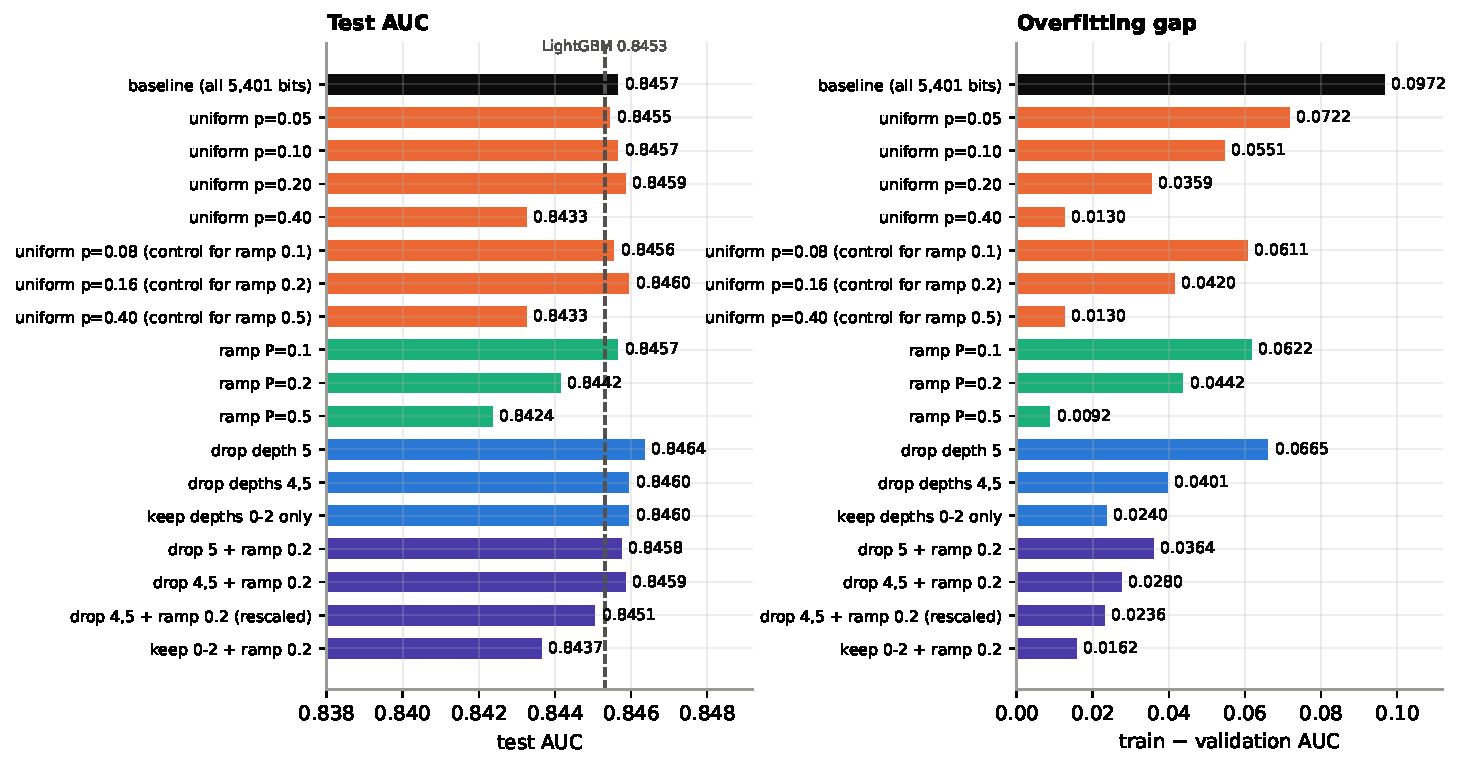
\includegraphics[width=\textwidth]{fig2_bars.pdf}
\caption{The same results as bars. Left: test AUC, with the LightGBM ceiling
dashed. Right: the overfitting gap. The left panel is nearly flat; the right
panel spans an order of magnitude.}
\end{figure}

\begin{figure}[h]\centering
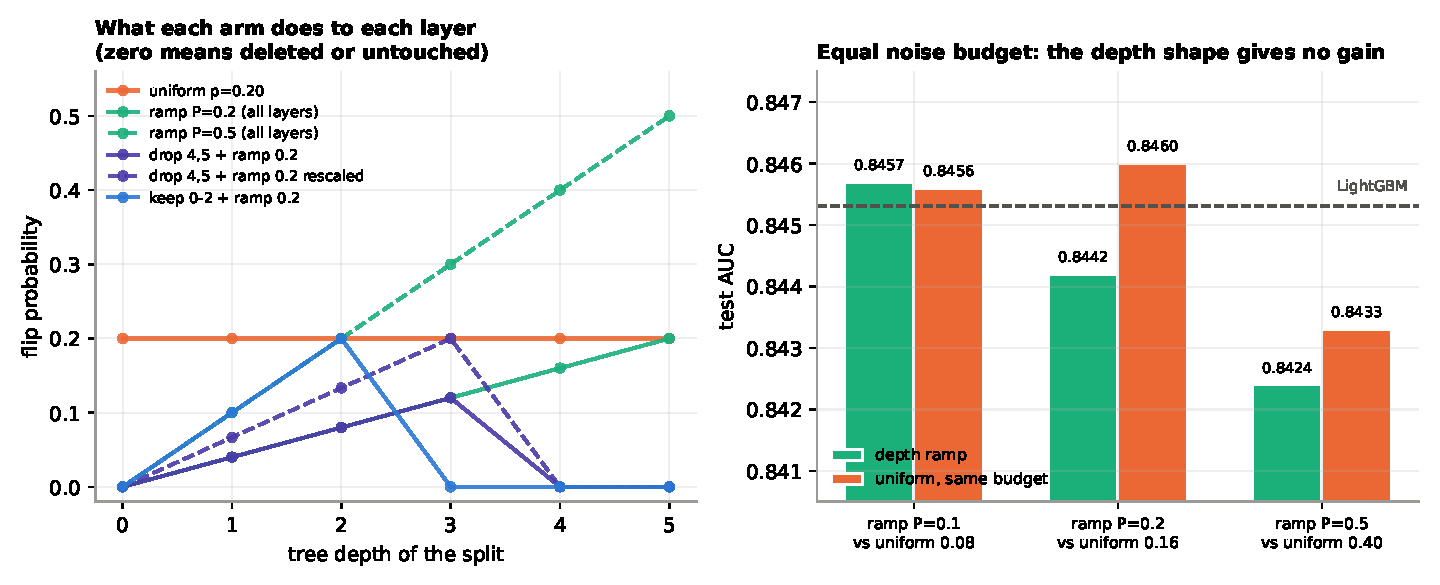
\includegraphics[width=\textwidth]{fig3_profile.pdf}
\caption{Left: the flip probability each arm applies at each depth; zero means
the layer was deleted or deliberately untouched. Right: each depth ramp beside
the uniform arm carrying the same average flip rate. At matched budget the ramp
never wins.}
\end{figure}

\clearpage
\section{Observations}

\begin{enumerate}

\item \textbf{Test AUC is almost completely insensitive to everything tried.}
Across all twenty-one configurations it spans \num{0.8424} to \num{0.8464}, a
range of \num{0.0040}, against a baseline of \num{0.8457}. For context, the
standard error of an AUC estimated on \num{2400} rows is approximately
\num{0.009}, so no arm is distinguishable from the baseline in absolute terms.
Thirteen of the eighteen configurations sit at or above the LightGBM ceiling.

\item \textbf{Overfitting, by contrast, is highly controllable.} The gap ranges
from \num{0.0972} at the baseline to \num{0.0092} under the heaviest ramp, a
reduction of \textbf{90.5\%}. The relationship with the noise level is
monotone: gaps of \num{0.0972}, \num{0.0722}, \num{0.0551}, \num{0.0359} and
\num{0.0130} for uniform flip rates of $0$, $0.05$, $0.10$, $0.20$ and $0.40$.

\item \textbf{Deletion is the most efficient regulariser.} Keeping only depths
0--2 uses \textbf{700 of 5{,}401 bits}, a 7.7-fold reduction, and yields test
AUC \num{0.8460} (baseline \num{0.8457}) with the gap cut from \num{0.0972} to
\num{0.0240}, a \textbf{75.3\% reduction}. It is also the fastest arm to fit,
\num{3.3}\,s against \num{48.7}\,s for the baseline. No noise is required to
achieve this.

\item \textbf{The depth shape of the noise provides no benefit at matched
budget.} Comparing each ramp with the uniform arm of the same average rate:
at $\bar p \approx 0.08$, \num{0.8457} versus \num{0.8456}; at $\bar p \approx
0.16$, \num{0.8442} versus \num{0.8460}; at $\bar p \approx 0.40$, \num{0.8424}
versus \num{0.8433}. The ramp is marginally behind in two of the three pairs and
level in the third. The hypothesis that deeper splits deserve more perturbation
is therefore \emph{not} supported once the total amount of noise is controlled
for.

\item \textbf{The combined design works, and works through deletion.} Dropping
depths 4 and 5 and ramping the survivors gives test AUC \num{0.8459} with a gap
of \num{0.0280}, a 71.2\% reduction, using \num{1480} bits. Decomposing it:
deletion alone accounts for a gap of \num{0.0401} and adding the ramp brings a
further \num{0.0121}. Both components help, deletion more than the ramp.

\item \textbf{Five arms fall below the tree ceiling, and four of them contain a
depth ramp.} They are ramp $P=0.5$ (\num{0.8424}), uniform $p=0.40$
(\num{0.8433}), keep 0--2 with a ramp (\num{0.8437}), ramp $P=0.2$
(\num{0.8442}) and drop 4,5 with the rescaled ramp (\num{0.8451}). Grouping the
configurations by whether they contain a ramp at all: the seven ramp arms
average \num{0.8447} with four below the ceiling, while the eleven non-ramp
arms average \num{0.8456} with one below. The two extreme-noise arms also have
the two smallest gaps, which shows the gap can be pushed past the useful point:
there the penalty is suppressing signal rather than memorisation.

\item \textbf{The raw features remain redundant.} Adding the ten original
columns to the full encoding changes test AUC from \num{0.8457} to \num{0.8454}
and the gap from \num{0.0972} to \num{0.0975}. This is the third independent
confirmation that the encoding subsumes the raw features.

\item \textbf{The measurements are stable.} Refitting three arms three times
each with fresh noise gave test-AUC spreads of \num{0.0001},
\num{0.0001} and \num{0.0002}. The ordering between arms is therefore
reproducible with respect to the noise draw, even though the absolute
differences are small.

\end{enumerate}

\section{Key findings}

\begin{enumerate}

\item \textbf{Overfitting in this model can be reduced by more than tenfold at
no cost in test accuracy.} This confirms and quantifies the premise of this
round. The gap is not a symptom that needs curing in order to improve
generalisation; it can be removed almost entirely while test AUC does not move.

\item \textbf{The recommended configuration is to keep only the three
shallowest tree layers.} Test AUC \num{0.8460} versus the LightGBM ceiling of
\num{0.8453}, overfitting gap \num{0.0240} instead of \num{0.0972}, and
\num{700} features instead of \num{5401}. It requires no noise, no extra
hyper-parameter and no stochastic training, and it fits about fifteen times
faster. If a slightly tighter gap is wanted at the same accuracy, dropping
depths 4 and 5 and ramping the survivors gives \num{0.8459} with a gap of
\num{0.0280}.

\item \textbf{Depth-targeted perturbation is not justified by these results.}
Once the total noise budget is matched, uniform flips do as well or slightly
better, and the pattern holds when the configurations are simply grouped: the
seven arms containing a ramp average \num{0.8447} in test AUC with four falling
below the tree ceiling, against \num{0.8456} and one for the eleven arms
without one. The intuition that deep splits are less reliable is correct as a
description of the encoding (they are fitted on roughly ten times fewer rows),
and \emph{deleting} them is indeed harmless, but \emph{graduating the noise by
depth} adds nothing over flipping everything equally and is mildly worse here.

\item \textbf{Test performance on this dataset is saturated and set by the
shallow tree structure.} Seven hundred bits from the top three layers extract
the full predictive content; the remaining \num{4701} bits contribute nothing to
generalisation and only provide capacity to memorise. Together with the earlier
finding that a linear model matches a 2.44-million-parameter network, the
picture is consistent: the quantity that determines accuracy here is the tree
structure in the encoding, not the model on top of it and not the amount of
regularisation applied to it.

\item \textbf{Practical consequence for the paper.} The method can be stated as
a logistic regression on a shallow, out-of-bag-honest tree encoding. It is
convex, has one hyper-parameter, trains in a few seconds, matches gradient
boosting on this dataset, and overfits four times less than the full encoding.
The next step required before any general claim is to repeat this on the other
clean datasets in the suite, since every number in this report comes from a
single dataset and a single split.

\end{enumerate}

\vfill
\noindent\rule{\textwidth}{0.4pt}\\
\begin{flushleft}\footnotesize
\textbf{Reproduction.}\\
Shared options for every arm:\\
\texttt{run\_feature\_reg.py -{}-task 361055 -{}-C 0.01 -{}-views tree -{}-encoding oob -{}-noise-copies 3}\\[2pt]
Per-arm flag added to the above:\\
\texttt{-{}-flip-uniform} \quad \texttt{-{}-flip-ramp} \quad \texttt{-{}-flip-ramp-rel}\\
\texttt{-{}-drop-layers} \quad \texttt{-{}-keep-layers} \quad \texttt{-{}-repeats}\\[2pt]
Driver notebook: \texttt{colab\_feature\_reg.ipynb}. All runs on CPU, random
seed \num{0}. Wall-clock time per fit ranged from \num{3.3}\,s (700 bits, no
noise) to \num{181.7}\,s (5{,}401 bits, three noisy copies).
\end{flushleft}

\end{document}
